Die Funktion
\[
\varphi(x)
=
\begin{cases}
0          &\qquad x \le -\frac{\pi}2 \\
\frac12a(1+\sin x)&\qquad -\frac{\pi}2<x\le \frac{3\pi}2\\
0          &\qquad \frac{3\pi}2\le x
\end{cases}
\]
ist die Wahrscheinlichkeitsdichte der Zufallsvariable $X$.
\begin{teilaufgaben}
\item
Bestimmen Sie $E(X)$.
\item
Wie muss $a$ gewählt werden, damit $\varphi(x)$ auch wirklich eine 
Wahrscheinlichkeitsdichte ist?
\item
Berechnen Sie $\operatorname{var}(X)$.
\end{teilaufgaben}

\begin{hinweis}
Versuchen Sie a) zu lösen ohne explizit ein Integral auszurechnen.
\end{hinweis}

\begin{center}
\def\p{3.14159}
\def\a{1.5}
\def\b{3}
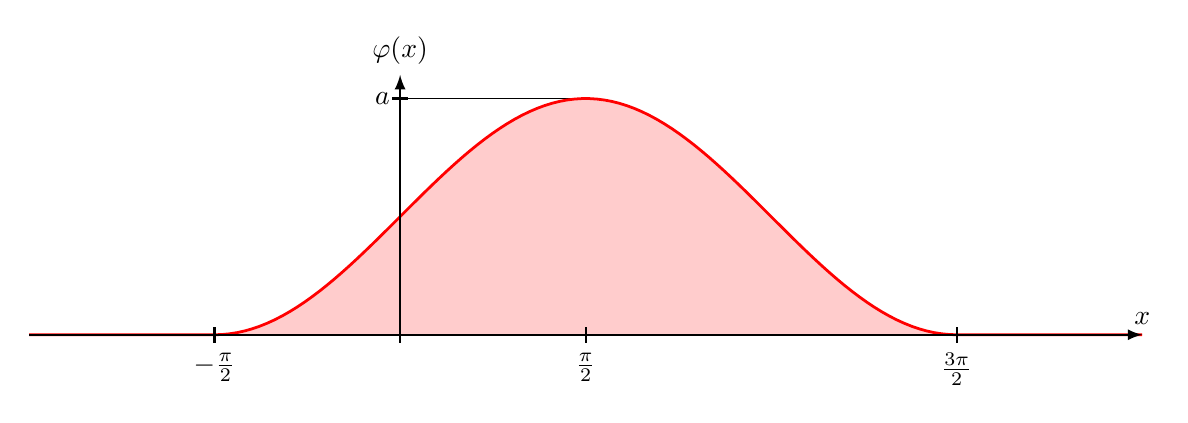
\begin{tikzpicture}[>=latex,thick]
\draw[line width=0.1pt] (0,{\b})--({0.5*\p*\a},{\b});
\fill[color=red!20] plot[domain={-0.5*\p}:{1.5*\p},samples=100] ({\x*\a},{0.5*(1+sin(180*\x/\p))*\b})--cycle;
\draw[color=red,line width=1pt] ({-\p*\a},0)--plot[domain={-0.5*\p}:{1.5*\p},samples=100] ({\x*\a},{0.5*(1+sin(180*\x/\p))*\b}) -- ({2*\p*\a},0);
\draw[->] ({-\p*\a},0) -- ({2*\p*\a},0) coordinate[label={$x$}];
\draw[->] (0,-0.1) -- (0,{1.1*\b}) coordinate[label={$\varphi(x)$}];
\draw (-0.1,{\b})--(0.1,{\b});
\draw ({0.5*\p*\a},-0.1) -- ({0.5*\p*\a},0.1);
\draw ({-0.5*\p*\a},-0.1) -- ({-0.5*\p*\a},0.1);
\draw ({1.5*\p*\a},-0.1) -- ({1.5*\p*\a},0.1);
\node at (0,{\b}) [left] {$a$};
\node at ({-0.5*\p*\a},{-0.1}) [below] {$-\frac{\pi}2$};
\node at ({0.5*\p*\a},{-0.1}) [below] {$\frac{\pi}2$};
\node at ({1.5*\p*\a},{-0.1}) [below] {$\frac{3\pi}2$};
\end{tikzpicture}
\end{center}



\begin{loesung}
\begin{teilaufgaben}
\item
Die Verteilung ist symmetrisch um $\frac{\pi}2$, also ist
$E(X)=\frac{\pi}2$.
\item
Es muss gelten
\begin{align*}
1
&=
\int_{-\infty}^{\infty}\varphi(x)\,dx
=
\int_{-\frac{\pi}2}^{\frac{3\pi}2} \frac{a}2(1+\sin x)\,dx
=
\frac{a}2\cdot \biggl(
\int_{-\frac{\pi}2}^{\frac{3\pi}2} 1\,dx
+
\int_{-\frac{\pi}2}^{\frac{3\pi}2} \sin x\,dx
\biggr)
\\
&=
\frac{a}2\cdot 2\pi
=
a\pi
,
\end{align*}
das zweite Integral fällt weg, da hier die Funktion $\sin x$ über eine
ganze Periode integriert wird.
Man liest daraus ab, dass  $a=1/\pi$.
\item
Für die Varianz brauchen wir den Erwartungswert $E(X^2)$:
\begin{align*}
E(X^2)
&=
\int_{-\infty}^{\infty} x^2\varphi(x)\,dx
=
\frac1{\pi}
\int_{-\frac{\pi}2}^{\frac{3\pi}2} x^2(1+\sin x)\,dx
=
\frac1{\pi}
\biggl[
\frac{x^3}3
+2x\sin x + (2-x^2)\cos x
\biggr]_{-\frac{\pi}2}^{\frac{3\pi}2}
\\
&=
\frac{7\pi^2-24}{12}
\\
\operatorname{var}(X)
&=
E(X^2)-E(X)^2
=
\frac{7\pi^2-24}{12}
-
\frac{\pi^2}{4}
=
\frac{\pi^2-6}{3} \simeq 1.28986813369645287289.
\qedhere
\end{align*}
\end{teilaufgaben}
\end{loesung}

\thema{Wahrscheinlichkeitsdichte}
\thema{Erwartungswert}
\thema{Varianz}

\begin{diskussion}
Den Wert von $a$ kann man ebenfalls ohne Berechnung eines Integrals
ermitteln.
Dazu beachtet man, dass die Sinus-Kurve punktsymmetrisch ist um die
Wendepunkte.
Die rote Kurve teilt daher das Rechteck mit
$-\frac{\pi}2 \le x\le \frac{3\pi}2$ und $0\le y\le a$ in zwei gleich
grosse Teilflächen.
Der Inhalt dieses Rechtecks ist $2\pi\cdot a$.
Damit die rote Fläche den Inhalt $1$ hat, muss also $2\pi a/2 = 1$ gelten
oder $a = 1/\pi$.
\end{diskussion}

\begin{bewertung}
Erwartungswert aus Symmetrie ({\bf E}) 1 Punkt,
Normierungsbedingung ({\bf N}) 1 Punkt,
Wert von $a$ ({\bf A}) 1 Punkt,
Integral für $E(X^2)$ ({\bf I}) 1 Punkt,
Wert des Integrals ({\bf W}) 1 Punkt,
Wert der Varianz ({\bf V}) 1 Punkt.
\end{bewertung}



